\documentclass[12pt]{article}
\usepackage[utf8]{inputenc}
\usepackage{amsmath, amssymb, url, float, graphicx, float}
\usepackage{algorithm, algpseudocode}
\usepackage[small,bf]{caption}
\usepackage{marginnote}
\usepackage[inner=1in, outer=2.5in, marginparsep=.5in, marginparwidth=1.5in]{geometry}

\usepackage{tikz}
\usetikzlibrary{arrows, positioning}

\newcommand{\norm}[1]{\left\|{#1}\right\|_2}
\newcommand{\tm}{\theta^\mathrm{max}}
\newcommand{\lagr}{\mathcal{L}}
\newcommand{\sinc}{\mathop{\mathrm{sinc}}}
\newcommand{\nnz}{\mathop{\bf nnz}}
\newcommand{\eps}{\varepsilon}
\newcommand{\complex}{\mathbf{C}}
\newcommand{\ii}{\mathbf{i}}
\newcommand{\id}{\mathbb{I}}
\newcommand{\efix}{e^\mathrm{fix}}
\newcommand{\ifix}{i^\mathrm{fix}}
\newcommand{\iinc}{i^\mathrm{inc}}
\newcommand{\tmax}{\theta^\mathrm{max}}
\newcommand{\tmin}{\theta^\mathrm{min}}
\newcommand{\gmax}{g^\mathrm{max}}
\newcommand{\gmin}{g^\mathrm{min}}
\newcommand{\smin}{s^\mathrm{min}}
\newcommand{\smax}{s^\mathrm{max}}
\newcommand{\kfix}{{k^\mathrm{fix}}}
\newcommand{\hp}{h^\mathrm{p}}
\newcommand{\qp}{q^\mathrm{p}}
\newcommand{\C}{\mathcal{C}}
\newcommand{\E}[1]{\mathbb{E}\left[#1\right]}
\newcommand{\lek}{\preceq}

\newcommand{\downto}{\downarrow}
\newcommand{\upto}{\uparrow}


\tikzstyle{box}=[draw, minimum size=1.5cm]
\tikzstyle{arr} = [thick,->,>=stealth]
\tikzstyle{arrb} = [thick, |--]

\renewcommand*{\marginfont}{\footnotesize}

\let\emptyset\varnothing

\input defs.tex

\bibliographystyle{alpha}

\title{Notes for HRP 204}
\date{Spring 2020}
\author{Guillermo Angeris}

\begin{document}

\maketitle

\section{Session 3 (April 14)}
The idea of this session is to add demography data in a (relatively) simple way
to the original SIR model.

\subsection{Definitions}

\paragraph{Survival curves.} The survival curve is a function which maps
the current age to its survival rate. (\ie, it takes in an age and outputs
the percentage of the population which survives to be greater than, or 
equal to this age. Another way of stating this is as the probability that
the age of death $X$ is greater than some given $\alpha$, $P(X \ge \alpha)$,
where $\alpha$ is the desired age.)

\paragraph{Mortality rate.} In the case that this curve follows an exponential
distribution, we will define the exponential parameter as the \emph{mortality
rate}, which we will write as $\mu \in \reals_+$.  This would then imply that
the area under the graph is the life expectancy, and would be equal to
$1/\mu$.\marginnote{This comes from the fact that $\E{X} = \int P(X \ge
x)\,dx$.} This also gives us a simple way of estimating the average mortality
rate for any given distribution by setting $\mu \approx 1/\E{X}$.

\subsection{Simple models}
The obvious `world's simplest model' is an easy one: let $S$ be the number of
susceptible individuals~\ref{fig:simplest-model} In this model, $S(t)$ is
always constant for all time (\ie, by definition $\dot S = 0$), and of course
has no interesting dynamics.

\begin{figure}[ht!]
\centering
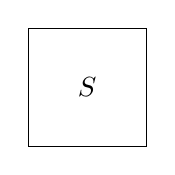
\begin{tikzpicture}
    \node [box](a) {$S$};
\end{tikzpicture}
\caption{World's simplest model.}
\label{fig:simplest-model}
\end{figure}

A slightly more complicated model (shown in
figure~\ref{fig:simple-model-deaths}) just includes the death rate as a `leaky
state.' In other words, the decay is given by $\dot S(t) = -\mu S(t)$, which has
the obvious solution
\[
    S(t) = S_0e^{-\mu t},
\]
a decaying exponential.

\begin{figure}[ht!]
\centering
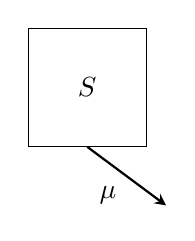
\begin{tikzpicture}
    \node [box](a) {$S$};
    \path (a.south) edge[arr] node[below left] {$\mu$} (1,-1.5);
\end{tikzpicture}
\caption{World's second simplest model.}
\label{fig:simple-model-deaths}
\end{figure}

Finally, an only slightly \emph{more} complicated model comes from adding
births (with rate $b \in \reals_+$) to the previous one (shown in
figure~\ref{fig:simple-model-births}). The result is the differential equation
$\dot S(t) = (b - \mu)S(t)$ with solution
\[
    S(t) = S_0e^{(b - \mu)t}.
\]
This is still an exponential (except when $b = \mu$, in which case the
population is constant).

\begin{figure}[ht!]
\centering
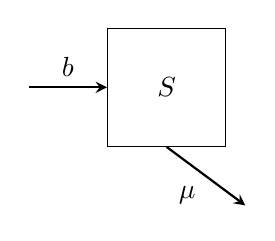
\begin{tikzpicture}
    \node [box](a) {$S$};
    \path (a.south) edge[arr] node[below left] {$\mu$} (1,-1.5);
    \path (-1.75, 0) edge[arr] node[above] {$b$} (a);
\end{tikzpicture}
\caption{World's third simplest model.}
\label{fig:simple-model-births}
\end{figure}

\subsubsection{Adding mortality in SIR}
Using the previous simple idea, we can then easily add death rates to the SIR
model.

\paragraph{Demography model.} A simple, basic assumption when adding birth
and death rates to the SIR model is to have the mortality rate be equal
for any of the three states, and, to prevent issues with normalization
we often assume that $\mu = b$.\marginnote{This ensures that the population is
always constant in  our model, so it can be normalized.} Note that this does
not include any excess mortality rates from the disease itself (we will deal
with this later). 


\begin{figure}[ht!]
\centering
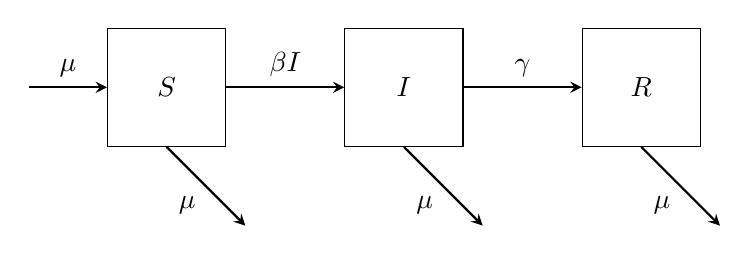
\begin{tikzpicture}[node distance=1.5cm, auto]
    \node [box](S) {$S$};
    \node [box, right=of S](I) {$I$};
    \node [box, right=of I](R) {$R$};

    \path (S.south) edge[arr] node[below left] {$\mu$} ++ (1,-1);
    \path (-1.75, 0) edge[arr] node[above] {$\mu$} (S);
    \path (I.south) edge[arr] node[below left] {$\mu$} ++ (1,-1);
    \path (R.south) edge[arr] node[below left] {$\mu$} ++ (1,-1);
    \path (S.east) edge[arr] node[above]{$\beta I$} (I);
    \path (I.east) edge[arr] node[above]{$\gamma$}(R);
\end{tikzpicture}
\caption{SIR incorporating deaths.}
\label{fig:sir-deaths}
\end{figure}

The new model equations (modeled in figure~\ref{fig:sir-deaths}) then are
\[
\begin{aligned}
    \dot S &= \mu - \beta IS - \mu S\\
    \dot I &= \beta IS - \gamma I - \mu I\\
    \dot R &= \gamma I  - \mu R.
\end{aligned}
\]

\paragraph{Simple properties.} We can give some simple thresholds and properties
of the system by analyzing interesting cases. For example, if infections are
`taking off,' then we must have
\[
    \dot I \ge 0 \implies \beta IS - \gamma I - \mu I \ge 0.
\]
Since $I \ge 0$ always, then we must have
\begin{equation}\label{eq:taking-off}
    \beta S - \gamma - \mu \ge 0 \implies S \ge \frac{\gamma + \mu}{\beta},
\end{equation}
\ie, that the susceptible proportion of the population must be greater than the
rate of recovery \emph{and} the rate of deaths and births divided by
$\beta$. We should note that this is larger than the SIR model without demographics since $\mu > 0$.\marginnote{Intuitively, this happens since we can view the total period of infectiousness as lasting roughly $1/(\gamma + \mu)$ rather than $1/\gamma$.}

With demography, we can then derive $R_0$ as the inverse of the susceptible
fraction
\[
    R_0 = \frac{\beta}{\gamma + \mu},
\]
which is always smaller than that of the non-demographic model.

\subsection{Equilibria}
We say a condition is at an \emph{equilibrium} if its relative proportions do not change
over time, \ie, if all time derivatives are zero. Additionally, we will say that
a disease is \emph{endemic} when it is at an equilibrium, but the infected
proportion is strictly positive.

\paragraph{Equilibria of SIR with demography.} To compute the equilibria,
we simply find $(S^*, I^*, R^*)$ such that
\[
    \dot S(t) = \dot I(t) = \dot R(t) = 0,
\]
simultaneously at these points. A rather simple and not terribly exciting
equilibrium is at $(S^*, I^*, R^*) = (1, 0, 0)$, \ie, no infections have
been introduced. We will call this the \emph{disease-free equilibrium}.

A second important equilibrium is the \emph{endemic equilibrium}, which happens
when, in the same way as~\eqref{eq:taking-off},
\[
    I^*(\beta S^* - \gamma - \mu) = 0,
\]
but, since $I^* > 0$ by assumption, we must have
\[
    S^* = \frac{1}{R_0},
\]
as defined above. This implies that the infected population must satisfy
\[
    0 = \mu - \beta I^*S^* - \mu S^* = \mu - \frac{\beta I^* - \mu}{R_0},
\]
so
\begin{equation}\label{eq:I-endemic}
    I^* = \frac{\mu(R_0 - 1)}{\beta}.
\end{equation}

\paragraph{Stability of equilibria.} While we will not prove this here, we can note that each of the two equilibria have certain ranges in which they are stable.\marginnote{In other words, if the system is at some equilibrium point, `pushing' the system by changing $S$, $I$, or $R$ in some way will cause the system to return back to its original equilibrium state.} If $R_0 < 1$, then the endemic equilibrium is infeasible (\ie, there does not exist an equilibrium point which satisfies both $I^* > 0$ \emph{and} $R_0 < 1$), which is easily seen from~\eqref{eq:I-endemic}. The only remaining equilibrium is the disease-free equilibrium, in which the disease eradicates itself since its reproduction rate is smaller than one, and this equilibrium point is always stable.

If $R_0 > 1$, then the disease-free equilibrium is always unstable. Introducing any nonzero proportion of infected causes the system to move towards the endemic equilibrium.\marginnote{There should be a simple, Lyapunov-style argument for this, but I haven't yet found it. Would be interesting to explore.} In particular, the system will have oscillatory behavior, and tend to an equilibrium point is exactly the endemic equilibrium.

\paragraph{Oscillatory behavior.} We will also not prove this here, but we can derive the approximate period of the oscillations of the system, when converging to the endemic equilibrium. In particular, we can show\marginnote{I'm curious about this. Do we assume an ansatz and derive the corresponding envelope?} that the period, $T$, of each oscillation is approximately:
\[
T \approx 2\pi\sqrt{AG},
\]
where $A$ is the average age of infection and $G$ is the average duration of infectiousness. We can given an approximate value of $A$ for an SIR + demography model, by using the fact that, in the endemic equilibrium, the average period spent as susceptible is around $\frac{1}{\beta I^*}$ (\ie, this is the average age at which a person is infected). Using~\eqref{eq:I-endemic}, we get the result.

\paragraph{Interesting results.} If vaccination is implemented, yet the reduction is not enough to reach the critical threshold of $R_0 \ll 1$, we get the result that the \emph{average age of infections increases}, since
\[
A \approx \frac{1}{\mu(R_0 - 1)},
\]
and reducing $R_0$ therefore increases $A$.

\subsection{SIR with demography and excess mortality}
There are several approaches to this. The simplest case is to add a term that includes the excess mortality (\ie, mortality rate) at the infectious stage.

A simpler (and the more common approach) is to include a term $\rho$ which is approximately the probability of dying at the infectious stage before either recovering or dying of natural causes---in this case, $\rho$ is called the \emph{case fatality rate} or CFR.

\paragraph{Model and consequences.} Adding mortality also has the side effect that the number of birth rates is no longer equal to the number of deaths. This implies that the model cannot simply be normalized by the population size. The resulting model, with the new addition of birth rates $\nu \in \reals_+$ and case fatality rates $\rho \in \reals_+$ is
\[
\begin{aligned}
	\dot S &= \nu - \beta IS - \mu S\\
	\dot I &= \beta IS - (\gamma + \mu) I - \frac{\rho}{1 - \rho}(\gamma + \mu) I\\
	\dot R &= \gamma I - \mu R.
\end{aligned}
\]
Under the (rather common) assumption that mortality occurs late in the infectious period, we can simplify the above dynamics slightly to
\[
\begin{aligned}
	\dot S &= \nu - \beta IS - \mu S\\
	\dot I &= \beta IS - (\gamma + \mu) I\\
	\dot R &= (1 - \rho)\gamma I - \mu R.
\end{aligned}
\]

\paragraph{Chronic infections.} There are several simple special cases of this model. For example, taking $\rho = 1$, yields the case of infections which persist until death. This includes long-term infections (\eg, HPV, HCV) or short-term infections with high fatality rates (\eg, Ebola, Mad Cow Disease). This model has the endemic equilibrium given by
\[
S^* = \frac{\nu}{\beta - \gamma}, \quad I^* = \frac{\nu(\beta - \gamma - \mu)}{(\beta - \gamma)(\gamma + \mu)},
\]
when $R_0 > \beta / (\gamma + \mu)$.\marginnote{It might be good to derive this at some point. Doesn't seem difficult, but may be a bit tedious.} 

\subsection{Other models}
\paragraph{Models without immunity.} A simple model is one where infectious individuals return to the susceptible pool rather than a separate `recovered' pool. This model is useful for infections which confer no immunity. The resulting equations are
\[
\dot S = \gamma I - \beta SI, \quad \dot I = \beta SI - \gamma I,
\]
with the endemic equilibrium given by
\[
S^* = \frac{\gamma}{\beta}, \quad I^* = 1 - \frac{\gamma}{\beta}.
\]

\paragraph{Model with rapidly waning immunity.} There is a second model, which generalizes the model without immunity, that follows from adding a term to the SIR + demography model which sends those recovered back into the susceptible pool (see figure~\ref{fig:sir-immunity}).
\begin{figure}[ht!]
\centering
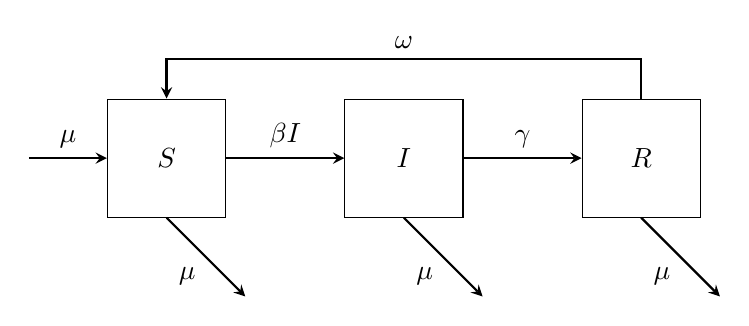
\begin{tikzpicture}[node distance=1.5cm, auto]
    \node [box](S) {$S$};
    \node [box, right=of S](I) {$I$};
    \node [box, right=of I](R) {$R$};

    \path (S.south) edge[arr] node[below left] {$\mu$} ++ (1,-1);
    \path (-1.75, 0) edge[arr] node[above] {$\mu$} (S);
    \path (I.south) edge[arr] node[below left] {$\mu$} ++ (1,-1);
    \path (R.south) edge[arr] node[below left] {$\mu$} ++ (1,-1);
    \path (S.east) edge[arr] node[above]{$\beta I$} (I);
    \path (I.east) edge[arr] node[above]{$\gamma$}(R);
    \draw[thick,->,>=stealth] (R.north) -- ++(0, .5) -| node[above,pos=.25]{$\omega$} (S.north);
\end{tikzpicture}
\caption{SIR incorporating deaths and waning immunity.}
\label{fig:sir-immunity}
\end{figure}
Note that, by sending $\omega \to 0$ we get the SIR + demography model, while sending $\omega \to +\infty$, we recover the model without immunity. The differential equations for this model are
\[
\begin{aligned}
	\dot S &= \mu - \beta IS - \mu S + \omega R\\
	\dot I &= \beta IS - (\gamma + \mu) I\\
	\dot R &= \gamma I - (\mu + \omega) R.
\end{aligned}
\]
As one might expect, the resulting oscillations are quite a bit more complex than those of the usual SIR + demography model.


\end{document}

